\documentclass[12pt, twoside]{article}
\usepackage[letterpaper, margin=1in, headsep=0.5in]{geometry}
\usepackage[english]{babel}
\usepackage[utf8]{inputenc}
\usepackage{amsmath}
\usepackage{amsfonts}
\usepackage{amssymb}
\usepackage{tikz}

\usepackage{pgfplots}
\pgfplotsset{width=9cm,compat=1.9}

\usepackage{venndiagram}

\usepackage{graphicx}
\usepackage{enumitem}
\usepackage{multicol}

\usepackage{fancyhdr}
\pagestyle{fancy}
\fancyhf{}
\renewcommand{\headrulewidth}{0pt} % disable the underline of the header

\fancyhead[LE]{\thepage}
\fancyhead[RO]{\thepage \\ Name: \hspace{4cm} \,\\}
\fancyhead[LO]{BECA / Dr. Huson / IB Mathematics\\* Unit 5: Polynomial functions\\* 29 January 2020}

\begin{document}
\begin{enumerate}[itemsep=0.5cm]
    \subsubsection*{5.1 Do Now: Function operations, algebra review, graphing quadratics}

    \item Let $f(x)=3x-4$ and $g(x)=5x$, for $x \in \mathbb{R}$.
    \begin{enumerate}[itemsep=1cm]
      \item Write down $g(-3)$.
      \item Find $(f \circ g)(x)$.
      \item Find $f^{-1}(x)$.\vspace{1.5cm}
    \end{enumerate}

    \item Let $f(x)=3x-1$ and $g(x)=-2x^2+2$
    \begin{enumerate}[itemsep=1.5cm]
        \item Find $f^{-1}(x)$.
        \item Find $(f \circ g)(1)$.\vspace{2.5cm}
    \end{enumerate}


\item The diagram below shows the graph of a function $f$, composed of four points.
\begin{multicols}{2}
    \begin{enumerate}[itemsep=0.5cm]
        \item Write down the value of $f(2)$.
        \item Write down the domain of $f$.
        \item Write down the range of $f$.
        \item Write down the value of $f^{-1}(1)$.
        \item Sketch the inverse of $f$, $f^{-1}$, on the grid at right. \vspace{0.5cm}
    \end{enumerate}
    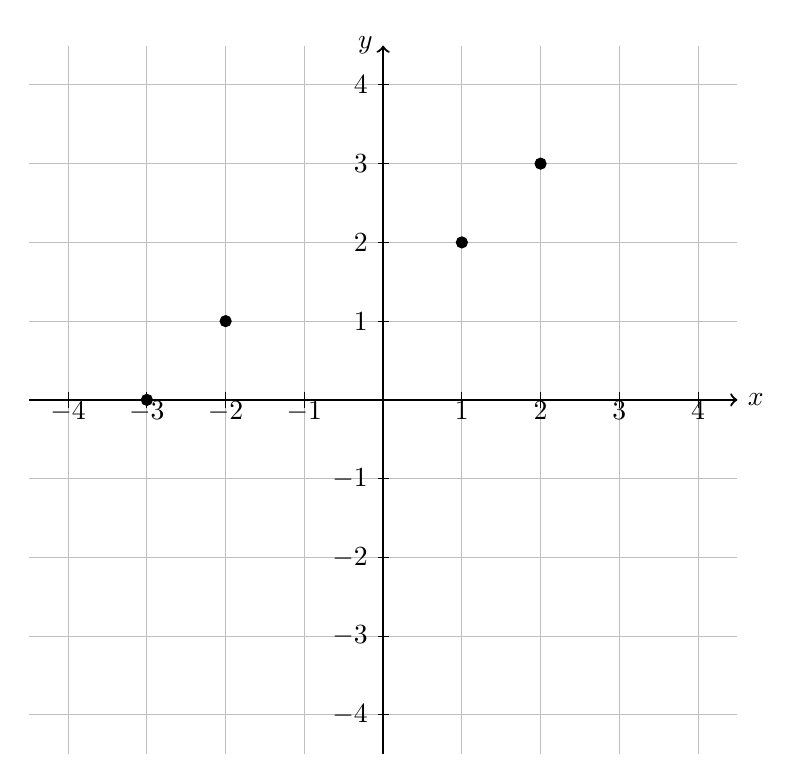
\begin{tikzpicture}
        \draw [thin, color=lightgray,, xstep=1.0cm,ystep=1.0cm] (-4.5,-4.5) grid (4.5,4.5);
        %\draw [thin, color=lightgray,, xstep=0.2cm,ystep=0.2cm] (-4.5,-1.5) grid (5.5,16.5);

        \foreach \x in {-4, -3, -2, -1,1,2,3,4}
        \draw[shift={(\x,0)},color=black] (0pt,-3pt) -- (0pt,3pt) node[below]  {$\x$};

        \foreach \y in {-4, -3, -2, -1, 1,2,3,4}
        \draw[shift={(0,\y)},color=black] (2pt,0pt) -- (-2pt,0pt) node[left]  {$\y$};

        \draw [thick, ->] (-4.5,0) -- (+4.5,0) node [right] {$x$};
        \draw [thick, ->] (0,-4.5) -- (0,4.5) node [left] {$y$};

        \draw (-3,0) circle[radius=2pt];
        \fill (-3,0) circle[radius=2pt];
        \draw (-2,1) circle[radius=2pt];
        \fill (-2,1) circle[radius=2pt];
        \draw (1,2) circle[radius=2pt];
        \fill (1,2) circle[radius=2pt];
        \draw (2,3) circle[radius=2pt];
        \fill (2,3) circle[radius=2pt];
    \end{tikzpicture}
\end{multicols}

\newpage
\subsubsection*{Quadratics algebra competencies} 
  
  \item Expand each binomial-squared expression to the form $ax^2+bx+c$.
  \begin{multicols}{2}
  \begin{enumerate}[itemsep=3cm]
    \item $(x+3)(x+3)$
    \item $(x+2)^2$ 
    \item $(x+5)^2$ 
    \item $(x+7)^2$ 
  \end{enumerate}
  \end{multicols}\vspace{3cm}
  
  \item Simplify each radical.
  \begin{multicols}{2}
    \begin{enumerate}[itemsep=2cm]
      \item $\sqrt{50}$ 
      \item $\sqrt{18}$
      \item $\sqrt{27}$ 
      \item $\sqrt{24}$ 
    \end{enumerate}
    \end{multicols}\vspace{2cm}
  
  \item Solve for the appropriate variable ($h$ and $r$).
    \begin{multicols}{2}
    \begin{enumerate}[itemsep=2cm]
      \item $Area=\frac{1}{2}(14.8)h=62.9$ 
      \item $Area=\pi r^2=483$ 
    \end{enumerate}
    \end{multicols}\vspace{2cm}

\newpage
\subsubsection*{Graphing quadratic functions (you may use a calculator)} 
    \item Consider the function $f(x)=x^2+2x-3$.
    \begin{enumerate}
        \item Sketch the graph of $f$, for $-4 \leq x \leq 2$. Label the vertex and the intercepts.
        \item This function can also be written in the form $f(x)=(x-p)^2 -4$.\\* 
        Write down the value of $p$. \vspace{1.5cm}
        \item The graph of $f$ has two solutions for $f(x)=0$. Write down the solutions (or roots, zeros) of the function. \vspace{1.5cm}
        \item Hence, write down the function in factored form, $f(x)=(x-a)(x-b)$. \vspace{1.5cm}
    \end{enumerate}
    \begin{center}
    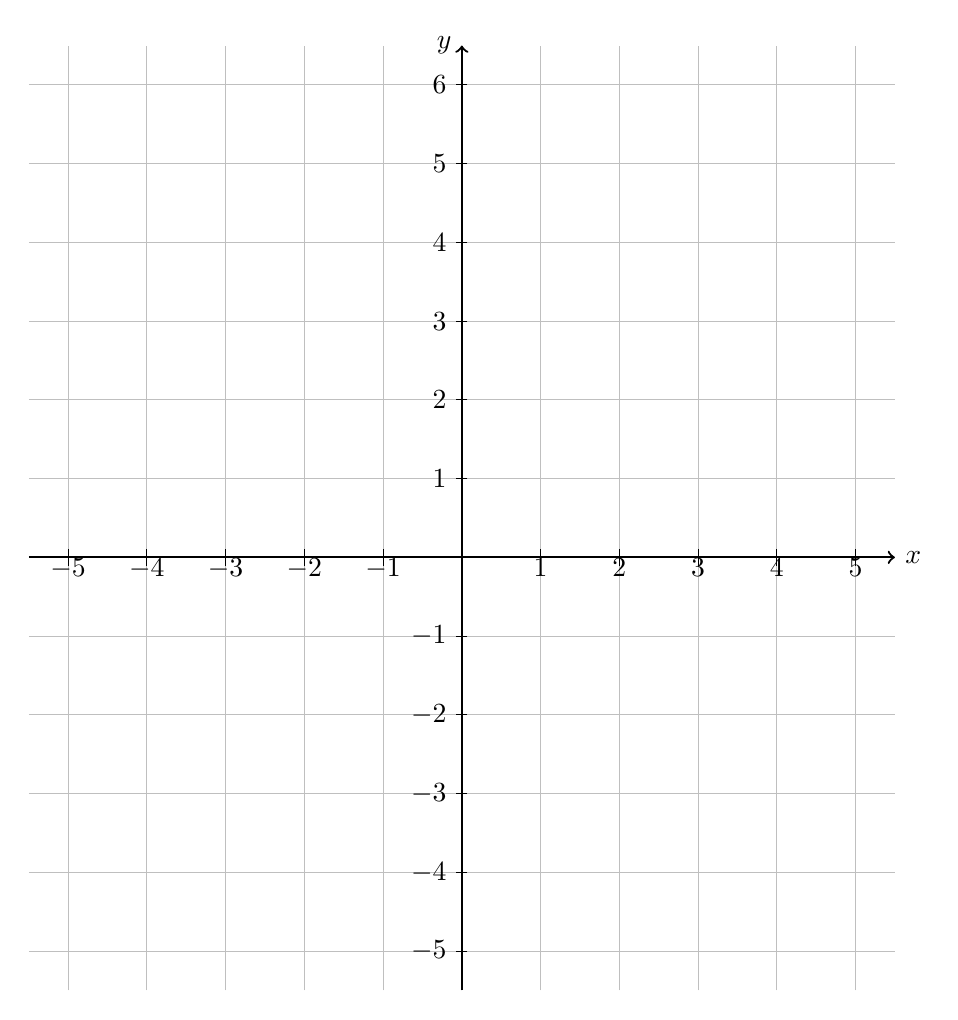
\begin{tikzpicture}
        \draw [thin, color=lightgray,, xstep=1.0cm,ystep=1.0cm] (-5.5,-5.5) grid (5.5,6.5);
        \foreach \x in {-5, -4, -3, -2, -1,1,2,3,4, 5}
        \draw[shift={(\x,0)},color=black] (0pt,-3pt) -- (0pt,3pt) node[below]  {$\x$};
        \foreach \y in {-5, -4, -3, -2, -1, 1,2,3,4, 5, 6}
        \draw[shift={(0,\y)},color=black] (2pt,0pt) -- (-2pt,0pt) node[left]  {$\y$};
        \draw [thick, ->] (-5.5,0) -- (+5.5,0) node [right] {$x$};
        \draw [thick, ->] (0,-5.5) -- (0,6.5) node [left] {$y$};
    \end{tikzpicture}
    \end{center}

\newpage
\subsection*{Sketching a quadratic function}
    \item   Given $f(x)=(x-3)^2-4$
    \begin{enumerate}[itemsep=0.9cm]
        \item Write down the vertex of the function as an ordered pair.
        %\item Write down the equation of the axis of symmetry.
        \item Expand the function from vertex form to standard form, $ax^2+bx+c \text{ where } a, b, c \;  \epsilon \; \mathbb{R}$. \vspace{1cm}
        \item Write down the value of $f(0)$. Explain what this represents on the graph. \vspace{1cm}
        \item Factor the function. Write down the roots. \vspace{1cm}
        \item Sketch the function, labeling the intercepts with values and the vertex as an ordered pair. Show the axis of symmetry as a dotted line and label it with its equation.
        \begin{center}
            \begin{tikzpicture}
                \draw [thick, ->] (-4.5,0) -- (+4.5,0) node [right] {$x$};
                \draw [thick, ->] (0,-3.5) -- (0,4.5) node [left] {$y$};
            \end{tikzpicture}
            \end{center}
        \item Write down the domain and range of the function.
    \end{enumerate}

\newpage
  \item Let $f$ be a quadratic function. Part of the graph of $f$ is shown below.\\*
  The vertex is at $P(2,1)$ and the $y$-intercept is at $Q(0, 3)$.\\*

    \begin{figure}[!htbp]
    \begin{center}
    \begin{tikzpicture}

        %grid
        %\draw [thin, color=lightgray,, xstep=1.0cm,ystep=1.0cm] (-5.5,-5.5) grid (5.5,5.5);
        %\draw [thin, color=lightgray,, xstep=0.2cm,ystep=0.2cm] (-5.5,-1.5) grid (5.5,16.5);

        \foreach \x in {-2, -1,1,2,3,4,5,6}
        \draw[shift={(\x,0)},color=black] (0pt,-3pt) -- (0pt,3pt) node[below]  {$\x$};

        \foreach \y in {-1,1,2,3,4,5,6}
        \draw[shift={(0,\y)},color=black] (2pt,0pt) -- (-2pt,0pt) node[left]  {$\y$};

        \draw [thick, ->] (-2.5,0) -- (+6.5,0) node [right] {$x$};
        \draw [thick, ->] (0,-1.5) -- (0,6.5) node [left] {$y$};

        \draw (2,1) circle[radius=2pt] node [below] {$P$};
        \fill (2,1) circle[radius=2pt];
        \draw (0,3) circle[radius=2pt] node [right] {$Q$};
        \fill (0,3) circle[radius=2pt];

        \draw [<->] plot[domain= -1:5] (\x, .5*\x*\x -2*\x +3);

    \end{tikzpicture}
    \end{center}
    \end{figure}

    \begin{enumerate}
        \item Write down the equation of the axis of symmetry.
        \item The function $f$ can be written in the form $f(x)=a(x-h)^2 +k$. \\*
        Write down the value of $h$ and of $k$.
        \item Find $a$.
    \end{enumerate}


\end{enumerate}
\end{document}